\section{The proposed scheme: FSL-AKE v3}\label{sec:scheme}

FSL-AKE v3 is a drone--server and server--cloud authenticated key agreement with key confirmation. \Cref{tab:rationale} lists
each design change, the findings it addresses and its cost effect; the full specification is \texttt{spec/fsl\_ake\_v3.md} of
the artifact. \Cref{fig:network} shows the entities.
\begin{figure}[!htbp]
\centering
\begin{tikzpicture}[node distance=1.2cm and 2.2cm, font=\small]
  \node[party] (ra) {RA};
  \node[party, below left=1.1cm and 1.6cm of ra] (de) {Drone $DE$};
  \node[party, below right=1.1cm and 1.6cm of ra] (es) {Ground station $ES$};
  \node[party, right=2.0cm of es] (cs) {Cloud server $CS$};
  \draw[dashed, black!60] (ra) -- node[above left, font=\scriptsize, pos=0.5, fill=white, inner sep=1pt] {registration} (de);
  \draw[dashed, black!60] (ra) -- node[above right, font=\scriptsize, pos=0.5, fill=white, inner sep=1pt] {registration} (es);
  \draw[msg, <->] (de) -- node[below, font=\scriptsize] {open channel: AKE, retry, data} (es);
  \draw[msg, <->] (es) -- node[below, font=\scriptsize] {AKE} (cs);
  \node[font=\scriptsize, below=0.15cm of de, align=center] {stores $TID, PID, K$};
  \node[font=\scriptsize, below=0.15cm of es, align=center] {stores $I(TID), I(PID)$, $C$, ticket;\\ $X_{ES}$ in a secure element};
  \node[font=\scriptsize, right=0.1cm of ra, align=left, text=black!70] {registers $DE$, $ES$;\\ erases what it issued};
\end{tikzpicture}
\caption{Network model. Dashed lines: registration over a secure channel. Solid arrows: open channels controlled by the
attacker. The stored values are those of \cref{sec:scheme}.}
\label{fig:network}
\end{figure}

\begin{table*}[!t]
\centering
\footnotesize
\caption{Design rationale (\texttt{spec/changes.json}). Each change, the findings it addresses (F: BAKMM-IoD, \cref{tab:flaws}; O, R: findings on the predecessor v2 and of our specification review, listed in the artifact) and its cost effect.}
\label{tab:rationale}
\setlength{\tabcolsep}{3pt}
\begin{tabular}{p{6.4cm}p{1.6cm}p{6.6cm}}
\toprule
Change (BAKMM-IoD / v2 $\rightarrow$ v3) & Flaws & Cost effect \\
\midrule
Hash with domain-separation labels & F2, F3 & none (label bytes inside the same hash call) \\
Server erases K at commit; one record per drone & F4, O2 & none for the commit itself \\
Retry ticket & O2, F7 & server +1 hash (E9) and +1 AES (E10) per session; drone +1 hash and +1 AES only on a retry \\
Keyed one-time retry pseudonym & F7, O9 & none: same hash call as TID' \\
Next identity hashed with K & F5, F9, F10 & none \\
Encrypted database index and record; no XOR & F8, F9, O3 & server: 2 hashes of the XOR mask of v2 replaced by AES operations (5 senc + 1 sdec per session in total) \\
Key confirmation message & O4 & +1 hash each side, +256 bits \\
No timestamps & O6 & -32 bits per message \\
Data record with counter under AEAD & F11 & 1 AES operation per record (as BAKMM-IoD's encryption), +64-bit counter, +128-bit tag \\
Session keys never stored; all field lengths checked & O5 & none \\
Check values V2, V3 computed from K, not from SK & R8 & none (same number of hashes) \\
\bottomrule
\end{tabular}
\end{table*}


\subsection{Equations}
Every computation is written once; both sides of every check use the same numbered equation. The equations below are
generated from the specification.
{\small% GENERATED from spec/fsl_ake_v3.md section 4 by paper/scripts/make_tables.py -- equations identical to the spec
\begin{multline*}\tag{E0}\label{eq:E0} X_{idx} = H(\text{``x-idx''}, X_{ES})[0..127]\;\text{,} \\ X_{db} = H(\text{``x-db''}, X_{ES})[0..127] \end{multline*}
\noindent{\footnotesize computed by: ES, once per boot}\par
\begin{multline*}\tag{E1}\label{eq:E1} I(id) = \mathrm{PRP}_{X_{idx}}(id) \\ \text{; being a permutation, ES reads}\;id\;\text{back as}\;\mathrm{PRP}^{-1}_{X_{idx}}(I(id)) \end{multline*}
\noindent{\footnotesize computed by: ES}\par
\begin{multline*}\tag{E2}\label{eq:E2} C = \mathrm{AEAD}_{X_{db}}(\nu ; K; \text{``rec''}  \|  dev)\;\text{,} \\ \nu \;\text{random, stored as}\;(\nu , C) \end{multline*}
\noindent{\footnotesize computed by: ES}\par
\begin{equation*}\tag{E3}\label{eq:E3} V_1 = H(\text{``v1''}, K, TID, N_1) \end{equation*}
\noindent{\footnotesize computed by: DE sends, ES checks}\par
\begin{equation*}\tag{E3r}\label{eq:E3r} V_{1r} = H(\text{``v1r''}, K, PID, N_{1r}) \end{equation*}
\noindent{\footnotesize computed by: DE sends, ES checks}\par
\begin{multline*}\tag{E4}\label{eq:E4} SK = H(\text{``sk''}, K, TID, n, N_2)\;\text{,} \\ n\;\text{=}\;N_1\;\text{(first attempt) or}\;N_{1r}\;\text{(retry)} \end{multline*}
\noindent{\footnotesize computed by: DE and ES}\par
\begin{equation*}\tag{E5}\label{eq:E5} V_2 = H(\text{``v2''}, K, TID, n, N_2) \end{equation*}
\noindent{\footnotesize computed by: ES sends, DE checks}\par
\begin{equation*}\tag{E6}\label{eq:E6} V_3 = H(\text{``v3''}, K, TID, n, N_2) \end{equation*}
\noindent{\footnotesize computed by: DE sends, ES checks}\par
\begin{equation*}\tag{E7}\label{eq:E7} K' = H(\text{``k''}, K, SK) \end{equation*}
\noindent{\footnotesize computed by: DE and ES}\par
\begin{multline*}\tag{E8}\label{eq:E8} W = H(\text{``id''}, K, TID, SK)\;\text{;} \\ TID' = W[0..159]\;\text{,} \\ PID' = W[160..255] \end{multline*}
\noindent{\footnotesize computed by: DE and ES}\par
\begin{equation*}\tag{E9}\label{eq:E9} R = H(\text{``r''}, K, TID, n)[0..127] \end{equation*}
\noindent{\footnotesize computed by: ES on every commit; DE only on a retry}\par
\begin{equation*}\tag{E10}\label{eq:E10} T = \mathrm{AEAD}_{R}(0^{96}; N_2; \text{``tkt''}) \end{equation*}
\noindent{\footnotesize computed by: ES; DE decrypts}\par
\begin{equation*}\tag{E11}\label{eq:E11} KD = SK[0..127] \end{equation*}
\noindent{\footnotesize computed by: DE and ES}\par
\begin{equation*}\tag{E12}\label{eq:E12} \text{data record}\;D = (ctr, \mathrm{AEAD}_{KD}(dir  \|  ctr; data; \text{``dat''}  \|  dir  \|  ctr)) \end{equation*}
\noindent{\footnotesize computed by: sender; receiver decrypts}\par
}

\subsection{Registration}
The RA picks $TID$, $PID$ and $K$ at random and a fresh device number $dev$, gives $(TID, PID, K)$ to the drone and
$(dev, TID, PID, K)$ to the ground station over a secure channel, and erases them (\cref{fig:registration}). The ground station
stores the indices $I(TID)$, $I(PID)$ (E1) and the record $(\nu, C)$ (E2).
\begin{figure*}[!t]
\centering
\begin{tikzpicture}
  \renewcommand{\msclen}{9.0}
  \mscstart{RA}{$DE$ and $ES$};
  \mscL[8.0cm]{pick $TID$ (160 bits), $PID$ (96 bits), $K$ (256 bits) and a fresh $dev$};
  \mscmsg{r}{to $DE$: $\{TID, PID, K\}$};
  \mscmsg{r}{to $ES$: $\{dev, TID, PID, K\}$};
  \mscR[8.0cm]{ES stores $I(TID)$, $I(PID)$ (E1) and $(\nu, C)$ (E2)};
  \mscL[8.0cm]{RA erases $K$, $TID$, $PID$};
  \mscend;
\end{tikzpicture}
\caption{Registration of FSL-AKE v3 (\texttt{spec/fsl\_ake\_v3.md}, \S6.1). Both arrows use the secure registration channel.}
\label{fig:registration}
\end{figure*}


\subsection{Drone--server authentication and key establishment}
\Cref{fig:ake} shows the three messages. The drone sends $MSG_1 = \{TID, N_1, V_1\}$. The ground station checks lengths, finds
the record by $I(TID)$, decrypts $K$ and checks $V_1$ (E3). It then picks $N_2$, computes $SK$ (E4), $V_2$ (E5), $V_3$ (E6),
$K'$ (E7), $TID'$ and $PID'$ (E8), $R$ (E9) and the ticket $T$ (E10), and commits atomically: it stores the new record over $K'$,
deletes the old record and the previous ticket, stores $T$ under the old index $I(PID)$, and erases $K$ and $R$. It sends
$MSG_2 = \{N_2, V_2\}$. The drone checks $V_2$ (E5), computes $SK$ (E4), and in one atomic step computes $V_3$, $K'$, $TID'$,
$PID'$, stores them and erases $K$, $TID$, $PID$ and $N_1$; it then sends $MSG_3 = \{V_3\}$. The ground station accepts $SK$
only if $V_3$ equals the pending value. The check values $V_2$ and $V_3$ are computed from $K$, so $SK$ enters no public value.
\begin{figure*}[!t]
\centering
\begin{tikzpicture}
  \mscstart{$DE$}{$ES$};
  \mscL{holds $TID, PID, K$; fresh $N_1$ (kept in non-volatile memory); $V_1$ (E3)};
  \mscmsg{r}{$MSG_1=\{TID, N_1, V_1\}$ \ (576 bits)};
  \mscR[9.2cm]{S1 lengths; S2 find record by $I(TID)$ (E1); S3 $K$ from $C$ (E2); S4 check $V_1$ (E3)\\
        S5 fresh $N_2$; $SK$ (E4), $V_2$ (E5), $V_3$ (E6), $K'$ (E7), $TID', PID'$ (E8), $R$ (E9), $T$ (E10)\\
        \phantom{S5 }\textbf{commit}: store record over $K'$; erase old record, $K$, $R$, previous ticket;\\
        \phantom{S5 }store $T$ under the old $I(PID)$; keep pending $(SK, V_3)$};
  \mscmsg{l}{$MSG_2=\{N_2, V_2\}$ \ (416 bits)};
  \mscL[9.2cm]{D2 lengths; check $V_2$ (E5); $SK$ (E4)\\
        D3 \textbf{atomic}: $V_3$ (E6), $K'$ (E7), $TID', PID'$ (E8); store them; erase $K, TID, PID, N_1$;\\
        \phantom{D3 }DE accepts $SK$};
  \mscmsg{r}{D4: $MSG_3=\{V_3\}$ \ (256 bits)};
  \mscR{S6 $V_3$ equals the pending $V_3$: ES accepts $SK$};
  \mscend;
\end{tikzpicture}
\caption{Drone--server authentication and key establishment of FSL-AKE v3 (\texttt{spec/fsl\_ake\_v3.md}, \S6.2). S1--S6 are server steps, D2--D4 drone steps ($MSG_3$ is sent at D4); equation
numbers as in \cref{sec:scheme}. Party indices are dropped ($DE$, $ES$). No timestamps are used. Total \BitsVthree\ bits.}
\label{fig:ake}
\end{figure*}


\subsection{Retry}
If the drone gets no $MSG_2$ it sends $MSG_{1r} = \{PID, N_{1r}, V_{1r}\}$ (E3r). If $I(PID)$ still indexes the record,
$MSG_1$ was lost and the ground station runs the normal steps with $n = N_{1r}$; if it indexes a ticket, $MSG_2$ was lost and
the ground station returns $T$ unchanged, from which the drone recovers $N_2$ with $R$ (E9) (\cref{fig:retry}). The drone keeps
$N_1$ and $N_{1r}$ in non-volatile memory until it has an answer and never replaces them before D3; if it loses them it must be
registered again. A second retry resends the same $MSG_{1r}$, so at most one retry per session can be unlinkable, and only when
every candidate drone lost $MSG_2$ (Tamarin, fixed scenario); it is linkable if $MSG_2$ is dropped for one drone only
(\cref{sec:discussion}).
\begin{figure}[!htbp]
\centering
\begin{tikzpicture}
  \mscstart{$DE$}{$ES$};
  \mscmsg{r}{$MSG_1=\{TID, N_1, V_1\}$ \ (576 bits)};
  \mscR[8.0cm]{S5: commit; ticket $T$ (E10) stored under the old index $I(PID)$};
  \msclost{l}{$MSG_2$ lost};
  \mscL{no answer: fresh $N_{1r}$; $V_{1r}$ (E3r)};
  \mscmsg{r}{$MSG_{1r}=\{PID, N_{1r}, V_{1r}\}$ \ (512 bits)};
  \mscR[9.0cm]{S2r: $I(PID)$ indexes a \emph{ticket} (case b): reply with $T$ unchanged\\ (the server cannot check $V_{1r}$: $K$ is erased)};
  \mscmsg{l}{$MSG_{2r}=\{T\}$ \ (288 bits)};
  \mscL[9.0cm]{D2r: $R$ (E9) with $N_1$; open $T$ (E10) to get $N_2$; $SK$ (E4); D3 as in \cref{fig:ake}};
  \mscmsg{r}{$MSG_3=\{V_3\}$ \ (256 bits)};
  \mscend;
  \node[comp=12.3cm, anchor=north west, font=\footnotesize] at ($(prev)+(0.15,-0.4)$) {%
    Case (a), $MSG_1$ lost: $I(PID)$ still indexes the record; ES checks $V_{1r}$ (E3r) and runs S3--S5 with $n=N_{1r}$.};
\end{tikzpicture}
\caption{Retry path of FSL-AKE v3 (\texttt{spec/fsl\_ake\_v3.md}, \S6.3), case (b), $MSG_2$ lost: at most one retry per session can be unlinkable (only when every candidate drone lost $MSG_2$). The keyed pseudonym $PID$ comes from E8
of the previous session.}
\label{fig:retry}
\end{figure}


\subsection{Server--cloud phase, data records and revocation}
The server--cloud phase uses the same messages and equations with the ground station as initiator, holding $\{TIN, PIN, K\}$,
and the cloud server as responder. Data records carry a counter under AEAD (E11, E12, \cref{fig:record}); the receiver
accepts a record only if it decrypts and its counter is larger than the last accepted one. Revocation deletes the record, both
indices and the ticket of a device.
\begin{figure}[!htbp]
\centering
\begin{tikzpicture}[font=\scriptsize, cell/.style={draw, minimum height=0.7cm, align=center}]
  \node[cell, minimum width=2.0cm, fill=lightgrey] (c) at (0,0) {$ctr$\\(64)};
  \node[cell, minimum width=5.0cm, right=0pt of c] (ct) {$\mathrm{AEAD}_{KD}$ ciphertext of $data$\\(length of $data$)};
  \node[cell, minimum width=2.2cm, right=0pt of ct] (tag) {tag\\(128)};
  \node[font=\scriptsize, below=0.35cm of ct, align=center] {nonce $= dir\,\|\,ctr$ (32 + 64 bits); associated data $= \text{``dat''}\,\|\,dir\,\|\,ctr$;\\
     $KD = SK[0..127]$ (E11); accepted only if the AEAD opens and $ctr$ is larger than the last accepted counter (E12)};
\end{tikzpicture}
\caption{Data-record format of FSL-AKE v3 (\texttt{spec/fsl\_ake\_v3.md}, \S6.5): \num{192} bits plus the data.}
\label{fig:record}
\end{figure}

